\documentclass[main.tex]{subfiles}

\begin{document}

\section*{Goal}
Today we will be investigating what is possibly one of the most utilized models in physics. The harmonic oscillator can be used to describe the vibrations of strings, the back-and-forth of a spring, the swing of a pendulum, the oscillation of atoms in a molecule, and many other periodic motions.

\section*{Equipment}
\begin{itemize}
\item
Force Sensor
\item
Photogate
\item
Motion Sensor
\item
Two Springs
\item
Dynamics Track and Cart
\item
Lab stand for Force Sensor
\item
Mass Bar for Cart
\item
Masses
\item
Triple-beam balance
\end{itemize}•

\section*{Theory}
We have used Hooke's Law several times this semester but have never studied the law itself in detail. To remind ourselves, Hooke's Law relates the force of an object attached to a spring with the displacement of the spring from what is called the equilibrium position as,
\begin{equation} \label{eq:Hooke}
\mathbf{F}=-k\mathbf{x},
\end{equation}
where $k$ is called the spring-force constant. The negative sign indicates that this is what is called a \emph{restoring} force meaning that the force is always directed towards the \emph{equilibrium position}---the point where the system has minimum potential energy.

As Hooke's Law is a force we can equate Equation~\eqref{eq:Hooke} to Newton's Second Law,
\begin{equation} \label{eq:AlgHarm}
ma=-kx.
\end{equation}
Equation~\eqref{eq:AlgHarm} is called the harmonic equation and in its standard form (and using differentials) is,
\begin{equation} \label{eq:Harmonic}
\frac{d^2x}{dt^2}+\frac{k}{m}x=0.
\end{equation}
With suitable choice of the zero of time, the general solution of Equation~\eqref{eq:Harmonic} can be written as follows,
\begin{equation}
x=A\cos(\omega t),
\end{equation}
where $\omega t$ ca be regarded as an angle, and the rate at which it increases is the so-called angular frequency,
\begin{equation}
\omega=\sqrt{\frac{k}{m}}.
\end{equation}
As the angular frequency $\omega$ is related to the (ordinary or ``cycles-per-second") frequency $\nu$ by,
\[
\omega=2\pi\nu,
\]
and frequency is related to the period $T$ by,
\[
T=\frac{1}{\nu},
\]
we can determine the period of oscillation by,
\begin{equation} \label{eq:Period}
T=\frac{1}{\nu}=\frac{2\pi}{\omega}=2\pi\sqrt{\frac{m}{k}}.
\end{equation}

For the first setup of our experiment we have two springs connected independently to the cart (borrowing a term from electronics, they are connected ``in parallel") the effective spring constant is the sum of the two individual spring constants, thus Equation~\eqref{eq:Period} is,
\begin{equation} \label{eq:2SpringPeriod}
T=2\pi\sqrt{\frac{m}{k_1+k_2}}.
\end{equation}

\section{Setup I: SHM of a Cart with Two Springs}
In this setup, the Force Sensor will measure the force that stretches each spring as it is pulled a short distance away from the Force Sensor. We will measure the amount of distance that the spring stretches and we will use Capstone to graph the force versus the distance. The slope of this line is the spring constant $k.$

Then we will use the Photogate to measure the motion of the cart that is oscillating back-and-forth as it is pulled by springs attached at each end. Capstone will calculate and display the period of oscillation which we can compare against our theoretical period.

\begin{enumerate}
\item
Open Capstone.
\item
Connect the Force Sensor to the 850UI and setup Capstone to read from it.
\item
Choose the ``Table \& Graph" template.
\item
For the first column in the table choose ``Force (N)" and for the second column click on ``$<$Select Measurement$>$" and under ``Create New" choose ``User-Entered Data." Name this User-Entered Data ``Distance" and give it units of ``m."
\item
Set up the graph so that the vertical axis measures ``Force (N)" and the horizontal axis measures ``Distance (m)."
\item
Put the five-pattern picket fence in the accessory tray of the cart so that the 2.5 cm single opaque band is at the top.
\item
Measure the mass of the cart and picket fence. Record this in the data table.
\item
Level the track by using the adjustable feet so that the cart will not roll one way or another.
\item
Mount the Force Sensor horizontally on a support rod at one end of the track.
\item
Attach an end stop to the end of the track that is opposite of the Force Sensor.
\item
Connect a spring to the end of the cart facing the Force Sensor using the small holes on the black end caps of the cart. Attach the other end of the spring to the Force Sensor's hook.

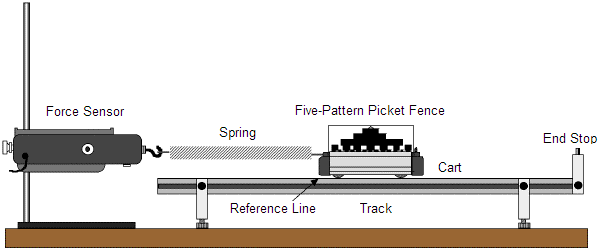
\includegraphics[width=\textwidth]{Harmonics_1_Setup}

\item \label{step:SpringConst_start}
Position the cart so the spring is in its relaxed length (neither stretched nor compressed). Put a mark on the track to indicate the initial position we will use this as a reference line for our readings.
\item
In Capstone, using the button next to the timer, change the recording mode from ``Continuous" to ``Keep." Click on ``Preview" to begin data collection.
\item
Press the tare button on the Force Sensor.
\item
With the cart in the correct position, enter the initial position of 0 m into the table and click on the ``Keep Sample" button to store the reading.
\item
Pull the cart 2 cm farther away from the Force Sensor. Hold the cart at this position then enter in the distance of 0.02 m into the table and click on ``Keep Sample."
\item
Continue to move the cart in 2 cm increments until the near edge of the cart is 24 cm from the reference line.
\item
Once at 24 cm, click on the Stop button to end the data collection.
\item \label{step:SpringConst_end}
Rescale the graph and apply a linear fit. The absolute value of the slope of the line is the spring constant for this spring. Record the spring constant in the data table as $k_1.$
\item
Disconnect the spring and replace it with the second spring. Make sure to keep track of which spring is which so we do not find the spring constant of the same spring twice.
\item
Repeat steps~\ref{step:SpringConst_start}--\ref{step:SpringConst_end} for the second spring. Record the spring constant of this spring as $k_2.$
\item
\textbf{Print} a copy of the graph showing both data sets (use the Select Data Run 
\includegraphics{Select_Data_Run} button to show both runs).
\end{enumerate}

\subsection*{Procedure}
\begin{enumerate}
\item
Unplug the Force Sensor then connect a Photogate to the 850UI.
\item
Open the file titled ``Harmonics1" by clicking on 
\includegraphics{Open_Experiment}. The file should be located in ..\textbackslash Documents\textbackslash Phys Lab Files\textbackslash Phys1154.
\item
Connect both springs to the cart and the end stops on the track.
\item
When the springs are attached at opposite ends of the track, the cart should be near the middle of the track.
\item \label{step:Harm1_start}
Position the Photogate so that it is aligned with the the center of the cart when the cart is at rest near the middle of the track. Adjust the height of the Photogate so the beam is blocked by the 2.5 cm opaque band at the top edge of the picket fence.
\item
Pull the cart about 25 cm from its equilibrium position at the middle of the track.
\item
Click on the Record button. Data collection should begin once the Photogate is first blocked.
\item
Release the cart so that it can move back-and-forth through the Photogate.
\item
After the cart completes eight or nine oscillations, click the the Stop button.
\item
The table will display the mean and standard deviation. Record these values in the data table.
\item \label{step:Harm1_end}
Measure the mass of the cart's extra mass bar. Record the mass in the data table.
\item
Add the mass bar to the cart and repeat steps~\ref{step:Harm1_start}--\ref{step:Harm1_end}.
\end{enumerate}

\subsection*{Analysis}
\begin{enumerate}
\item
Calculate the theoretical periods (Equation~\eqref{eq:2SpringPeriod}) and enter the results in the table provided. 
\item
Calculate the percent discrepancies for each run.
\end{enumerate}•

\section{Setup II: SHM of a Mass on a Spring}
In this setup, a Motion Sensor will measure the motion of a mass that is suspended from the end of the spring. Capstone will record the motion and display the position and velocity of the oscillating mass. The period of oscillation is then measured and compared to the theoretical value.

\begin{enumerate}
\item
From Setup I we have measured the spring constants of both springs. Choose one and copy the spring constant for that spring onto the data sheet for this setup.
\item
Start a new activity 
\includegraphics{New_Experiment} to clear all data from the previous setup.
\item
Remove all equipment from the previous setup then connect a Motion Sensor  and setup Capstone to record from it.
\item
Create a graph then add a second plot area 
\includegraphics{Add_New_Plot}. Select the top graph to measure Position and the bottom graph to measure Velocity.
\item
Using a support rod and clamp, suspend the spring so that it can move freely up and down.
\item
Put a mass hanger on the end of the spring, then add about 200 g to the hanger. Enough so that the spring will oscillate in a smooth motion. Record the total mass attached to the spring on the data sheet.
\item
Place the Motion Sensor on the floor directly below the mass hanger.
\item
Adjust the height of the spring so that the minimum distance from the mass hanger to the Motion Sensor is greater than 20 cm at the bottom of the mass hanger's movement.
\end{enumerate}•
\subsection*{Procedure}
\begin{enumerate}
\item
Pull the mass down about 5--10 cm then release it. Let it oscillate a few times so that any unwanted motion can dampen out.
\item
Click on the Record button to begin data collection. Continue recording for about 10 seconds then click on the Stop button to end data collection.
\end{enumerate}
n.b., If the data points do not appear on the plots for position and velocity, click on the rescale button 
\includegraphics{Rescale}. The position curve should resemble the plot of a sine function. If it does not, check the alignment of the Motion Sensor and the bottom of the mass hanger at the end of the spring. You may need to increase the reflecting area of the mass hanger by attaching a circular paper disk (about 6 cm diameter) to the bottom of the mass hanger. Erase the bad data set and repeat the data collection.

\subsection*{Analysis}
\begin{enumerate}
\item
Rescale the data as necessary.
\item
Use the Coordinates Tool 
\includegraphics{Coordinates_Tool} to find the average period of oscillation of the masses. Move the tool to the first peak of the Position vs Time graph, record the time value into the data table.
\item
Move the Coordinates Tool to each consecutive peak in the plot and record the time value.
\item
Find the period of each oscillation by calculating the difference between the times for each consecutive peak. Find the average of the periods. Record the result in the data table.
\item
Calculate the theoretical period using Equation~\eqref{eq:Period}.
\item
Calculate the percent discrepancy between the experimental and theoretical results.
\end{enumerate}•

\begin{samepage}
\hrulefill \\
\emph{Chapter~\ref{chap:Harmonics}:} \textbf{Simple Harmonic Motion}
\begin{enumerate}
\item
\textbf{(50)} Complete worksheet, showing sample calculations for all quantities.
\end{enumerate}•
\end{samepage}

\newpage
\section{Simple Harmonic Motion Worksheet}
\begin{flushright}
Name:\rule[-1mm]{5cm}{.1pt}
\end{flushright}•

\subsection*{Setup I}


Write the procedure for finding the spring constant.
\\[10cm]

\begin{enumerate}
\item
Do the theoretical values of the periods agree within one standard deviation of the experimental periods? Within two standard deviations?
\\[2cm]

\item
Does the period change with mass as the theoretical formula indicates? In what way? (Describe the nature of the dependence on mass.)
\end{enumerate}•
\newpage

\subsection*{Setup II}

\begin{enumerate}
\item
How does your calculated value for the period of oscillation compare to the measured value for the period of oscillation? Find the percent discrepancy between your calculated value and measured value.
\\[3cm]

\item
When the position of the mass is farthest from the equilibrium position, what is the velocity of the mass?
\\[3cm]

\item
When the absolute value of the velocity of the mass is greatest, where is the mass relative to the equilibrium position?
\end{enumerate}
\newpage

\section*{Data Tables}
\subsection*{Setup I}

\begin{doublespace}
\begin{tabular}{|l|@{\hskip 2cm}r|}
\hline
Item & Value\\
\hline
Mass of Cart & kg\\
\hline
Mass of Mass Bar & kg\\
\hline
Spring Constant $k_1$ & N/m\\
\hline
Spring Constant $k_2$ & N/m\\
\hline
Exp. Period (cart alone) & s\\
\hline
Std. Dev. (cart alone) & s\\
\hline
Exp. Period (cart \& mass) & s\\
\hline
Std. Dev. (cart \& mass) & s\\
\hline
\end{tabular}•
\\[2cm]

\begin{tabular}{l|r|}
\cline{2-2}
& Theoretical Period\\
\hline
\multicolumn{1}{|l|}{Cart} & s\\
\hline
\multicolumn{1}{|l|}{Cart \& Mass Bar} & s\\
\hline
\end{tabular}•

\newpage
\subsection*{Setup II}

Spring Constant $k=\rule[-1mm]{2.5 cm}{.1pt}$ N/m\\ \\
Hanging mass = \rule[-1mm]{2.5cm}{.1pt} kg
\\[1cm]

\begin{tabular}{|l|l@{\hskip 1cm}|l@{\hskip 1cm}|l@{\hskip 1cm}|l@{\hskip 1cm}|l@{\hskip 1cm}|l@{\hskip 1cm}|l@{\hskip 1cm}|}
\hline
Peak \# & 1 & 2 & 3 & 4 & 5 & 6 & 7\\
\hline
Time (s) &&&&&&&\\
\hline
Period (s) &\multicolumn{1}{|c|}{\Vhrulefill}&&&&&&\\
\hline
\end{tabular}•
\\[1cm]
\noindent
Average Period of Oscillation=\rule[-1mm]{2.5cm}{.1pt} s\\ \\
Calculated Period of Oscillation = \rule[-1mm]{2.5cm}{.1pt} s\\ \\
Percent Discrepancy = \rule[-1mm]{2.5cm}{.1pt}
\end{doublespace}
\end{document}
